\section{Homology of configuration spaces of surfaces}
\label{sec:HBraidSurf}
We want to study $H_*(\bms)=H_*(\cms)$,
which appears as the homology of the fiber
in the Leray-Serre spectral sequence associated to
\eqref{eq:Birman}, \eqref{eq:Birmanbundle} or \eqref{eq:BirmanbundleD}.
In particular we are interested in $H_*(C_m(\S))$
as a $\Z_2$-representation of the group $\gg$.

In \cite{LM} L\"offler and Milgram implicitly proved that $H_*(\bms)=H_*(\cms)$ is a $\Z_2$-symplectic
representation of the mapping class group. By \emph{$\Z_2$-symplectic} we mean the following:
\begin{defn}
 \label{defn:symplrep}
 Let $\H=H_1(\S)\simeq\Z_2^{2g}$.
 The natural action of $\gg$ on $\H$ induces a surjective map
 $\gg\to Sp_{2g}(\Z_2)$. A representation of $\gg$ over $\Z_2$ is called \emph{$\Z_2$-symplectic}
 if it is a pull-back of a representation of $Sp_{2g}(\Z_2)$ along this map.
\end{defn}

In \cite{BCT} B\"odigheimer, Cohen and Taylor computed $H_*(\cms)$ \emph{as a graded $\Z_2$-vector space}.
Their method provides all Betti numbers, but the action of $\gg$ cannot be easily deduced:
their descripition of $H_*(\cms)$ depends on a handle decomposition of $\S$, which is not preserved
by diffeomorphisms of $\S$, not even up to isotopy.

In this section and in the next one we will prove the following theorem; to the best of the author's knowledge
it does not appear in the literature.
\begin{thm}
 \label{thm:Hbms*as*ggrep}
 There is an isomorphism of bigraded $\Z_2$-representations of $\gg$
 \[
  \bigoplus_{m\geq 0} H_*\pa{\cms}\cong \Z_2\left[Q^j\epsilon\,|\, j\geq 0\right]\otimes\Sym_{\bullet}(\H).
 \]
 Here we mean the following:
 \begin{itemize}
  \item[(i)] on the left-hand side the bigrading is given by homological degree $*$ and by the direct summand,
  indexed by $m$,
  on which the homology class is supported, i.e. by the number $m$ of points
  involved in constructing the homology class; we call $*$ the \emph{degree} and $m$ the \emph{weight},
  and write $(*,m)$ for the bigrading;
  \item[(ii)] for $j\geq 0$, $Q^j\epsilon$ is the image in $H_{2^j-1}(C_{2^j}(\S))$ of a generator
  of the group $H_{2^j-1}(C_{2^j}(\D))\simeq \Z_2$ 
  under the natural map induced by the embedding $\D\hookrightarrow\mrS$,
  and $\Z_2\left[Q^j\epsilon\,|\, j\geq 0\right]$ is the polynomial ring on
  infinitely many variables $\epsilon,Q\epsilon,Q^2\epsilon,\dots$;
  \item[(iii)] $\H=H_1(\sg)$ is identified with $H_1(C_1(\S))$ in a natural way, and lives in degree $1$ and weight $1$;
  $\Sym_{\bullet}(\H)$ denotes the symmetric algebra on $\H$;
  \item[(iv)] degrees and weights are extended on the right-hand side by the usual multiplicativity rule;
  \item[(v)] the action of $\gg$ on the right is the tensor product of the trivial action
  on the factor $\Z_2[Q^j\epsilon\,|\, j\geq 0]$, and of the action on
  $\Sym_{\bullet}(\H)$ which is induced by the $\Z_2$-symplectic action on $\H$.
  \end{itemize}
\end{thm}
Note that for any bi-homogeneus element in the right-hand side, the weight is greater or equal than
the degree: indeed factors of the form $Q^j\epsilon$ have weight strictly higher than their degree,
whereas factors belonging to $\H$ or to its symmetric powers have equal weight and degree.
  
Note that in the case $g=0$ the group $\Gamma_{0,1}$ is trivial and the previous theorem
reduces to equation \eqref{eq:Cohen}.

We point out that in \cite{BoT} B\"{o}digheimer and Tillmann have essentially proved that for a field
$\mathbb{F}$ of any characteristic the $\mathbb{F}$-vector space
\[
  \bigoplus_{m\geq 0} H_*\pa{\cms;\mathbb{F}}
\]
is isomorphic, as a bigraded $\gg$-representation over $\mathbb{F}$, to the tensor product
of the ring $\mathbb{F}[\epsilon]$, with trivial action, and some other bigraded representation:
here $\epsilon$ denotes, in analogy with the notation of Theorem \ref{thm:Hbms*as*ggrep}, the standard generator of $H_0(C_1(\D))$.

% isomorphism of bigraded vector spaces
% \begin{equation}
% \label{eq:genuszero}
% \bigoplus_{m\geq 0} H_*\pa{C_m(\D)}\simeq \Z_2[Q^j\epsilon\,|\, j\geq 0].
% \end{equation}
% This isomorphism was essentially proved by Fuchs in \ref{Fuchs:CohomBraidModtwo}. Moreover the left hand
% side is the homology of the space $\coprod_{m\geq 0} C_m(\D)$, which has a natural structure
% of algebra over the operad $E^2$ of little $2$-cubes. The isomorphism in equation \eqref{eq:genuszero}
% is an isomorphism of rings (using the Pontryagin product on the left hand side), and $Q$ represents here
% the Araki-Kudo-Dyer-Lashof operation $Q\colon H_*(X;\Z_2)\to H_{2*+1;\Z_2}(X)$,
% which is defined for any $E^2$-algebra $X$; $\epsilon\in H_0(C_1(\D))$ is the generator.
% This explains our notation; we refer to Cohen \cite[Chap.3]{CLM} for more details.

In this section we will prove that there is an isomorphism of \emph{bigraded $\Z_2$-vector spaces}
as in Theorem \ref{thm:Hbms*as*ggrep}; in the next section we will deal with the action of
$\gg$.
%In these two sections we abbreviate $\S=\sg$.

Since we work with coefficients in a field, it is equivalent to compute homology or cohomology,
and in this section we will prefer to compute $H^*(\cms)$ for all bigradings $(*,m)$.
% the dual graded vector space $H_*(\cms)$ is abstractly isomorphic,
% i.e. it has the same dimension.

We will mimic the method used by Fuchs \cite{Fuchs:CohomBraidModtwo} to compute the $\Z_2$-cohomology
of $C_m(\D)$.
As already mentioned in Section \ref{sec:Preliminaries}, our computation recovers a known result, but it has the advantage of
being quite elementary and of providing a part of
the geometric insight that we will need in the next section.

In the whole section we assume $m\geq 0$ to be fixed.
Since the space $\cms$ is homeomorphic to the interior of a compact
$2m$-manifold with boundary, by Poincaré-Lefschetz
duality we have
\[
 H^*(\cms)\simeq \tilde H_{2m-*}(\cms^{\infty}),
\]
where in the right hand side we consider reduced homology of the one-point compactification (see Definition \ref{defn:opc}).

We introduce a space $\T(\S)$ which is homeomorphic to $\mrS$, the interior of $\S$. The construction
corresponds to a handle decomposition of $\S$ with one $0$-handle and $2g$ $1$-handles.

\begin{defn}
\label{defn:TS}
If $g=0$, hence $\S=\Sigma_{0,1}$ is the disc, we set $\T(\S)=]0,1[^2$, the interior of the unit square. Assume
now $g\geq 1$, and see Figure \ref{fig:defTS} to visualize the following construction.

Dissect the interval $[0,1]$ into $2g$ equal subintervals through the points $\cP_i=\frac{i}{2g}$ for $0\leq i\leq 2g$
(for $i=0,2g$ we get the two endpoints of $[0,1]$).

Consider on the vertical sides of $[0,1]^2$ the intervals
$I_i^l=\set{0}\times [\cP_i,\cP_{i+1}]$ and $I_i^r=\set{1}\times [\cP_i,\cP_{i+1}]$ for $1\leq i\leq 2g$:
all these intervals are
canonically diffeomorphic
to $[0,1]$ by projecting on the second coordinate, rescaling linearly by a factor $2g$
and translating.

We define a bijection
between the two sets of left and right intervals:
for $1\leq i\leq g$, the interval $I^l_{2i-1}$ corresponds to $I^r_{2i}$,
and the interval $I^r_{2i-1}$ corresponds $I^l_{2i}$.

The space $Q(\S)$ is the quotient of the square $[0,1]^2$ obtained by identifying each couple
of corresponding intervals in the canonical way. For $1\leq i\leq g$ we call $\overline{\U}_i$ the image
of $I^l_{2i-1}$ in the quotient $Q(\S)$, and we call $\overline{\V}_i$ the image of $I^l_{2g}$ in $Q(\S)$.

Note that the image in $Q(\S)$ of the set $\set{0,1}\times\set{\cP_0,\dots,\cP_{2g}}$ consists of two
points $\cP_{odd}$ and $\cP_{even}$: for $\epsilon\in\set{0,1}$ and $0\leq i\leq 2g$ the point
$(\epsilon,\cP_i)$ is mapped to $\cP_{even}$ if $\epsilon+i$ is even, and is mapped to $\cP_{odd}$
otherwise.

The spaces $\overline{\U}_i\subset Q(\S)$ and $\overline{\V}_i\subset Q(\S)$ are intervals with endpoints $\cP_{even}$ and $\cP_{odd}$;
the interiors of these intervals are disjoint. Each $\overline{\U}_i$ and $\overline{\V}_i$ is the homeomorphic image of
some left interval $I^l_j$, and inherits from the latter a parametrisation by $[0,1]$.

We call $\U_i$ and $\V_i$ the interiors of the intervals $\overline{\U}_i$ and $\overline{\V}_i$ respectively.

The space $Q(\S)$ is homeomorphic to the compact surface $\S$; we call $\T(\S)$ the interior of
$Q(\S)$.

From now on we will identify $\S$ with $Q(\S)$ and $\mrS$ with $\T(\S)$;
consequently we will identify $\cms$ with the
space of configurations of $m$ points in $\T(\S)$.
\end{defn}

\begin{figure}\centering
 \includegraphics[scale=0.7]{figures/defTS.pdf}
 \caption{The space $Q(\S)$ for $\S=\Sigma_{3,1}$. The black pentagons represent the point $\cP_{even}$, whereas the black
 squares represent $\cP_{odd}$.}
\label{fig:defTS}
\end{figure}


Our next aim is to define a structure of $CW$-complex on the space $\cms^{\infty}$:
the only $0$-cell will be the point $\infty$, whereas the other cells will be introduced
in the following definition.
\begin{defn}
\label{defn:ehopen}
A \emph{tuple} $\tup$ is a choice of the following set of data:
 \begin{itemize}
  \item a natural number $0\leq l\leq m$;
  \item a vector $\ux=(x_1,\dots, x_l)$ of integers $\geq 1$;
  \item vectors $\uu=(u_1,\dots,u_g)$ and $\uv=(v_1,\dots,v_g)$ of integers $\geq 0$,
 \end{itemize}
satisfying the following equality
\[
 m=\sum_{i=1}^lx_i+\sum_{i=1}^g(u_i+v_i).
\]
% We will generically use the letter $m$ to denote any of the numbers $l$, $x_i$,$y_i$,$z$,$u_i$,$v_i$ or $w_i$
% in the above sum, so $m\in\Z$; instead .
% Similarly we will use the letter $\M$ to denote any of the intervals $\U_i,\V_i,\W_i$;
% they will correspond to the letters $U_i,V_i,W_i$, so we also define a subset
% $\bsymb=\set{(U_i,V_i)_{i\leq g},(W_i)_{i\leq n-1}}\subset\symb$.
In symbols we write $\tup=(l,\ux,\uu,\uv)$. We omit from the notation $\ux$ if it vanishes: this happens precisely when $l=0$.
The \emph{dimension} of $\tup$ is defined as $m+l$.

For a tuple $\tup$ let $e^{\tup}$ be the subspace
of $\cms$ of configurations of $m$ points in $\mrS$ such that the following conditions hold
(see picture \ref{fig:defetup}):
\begin{itemize}
 \item for all $1\leq i\leq g$, exactly $u_i$ points lie on $\U_i$
 and exactly $v_i$ points lie on $\V_i$;
 \item there are exactly $l$ vertical lines in the open square $]0,1[^2\subset\mrS$ of the
 form $\set{s_i}\times]0,1[$ for some $0<s_1<\dots<s_l<1$, containing at least one
 point of the configuration. From left to right, these lines contain exactly $x_1,\dots,x_l$ points
 respectively.
\end{itemize}
\end{defn}


\begin{figure}\centering
 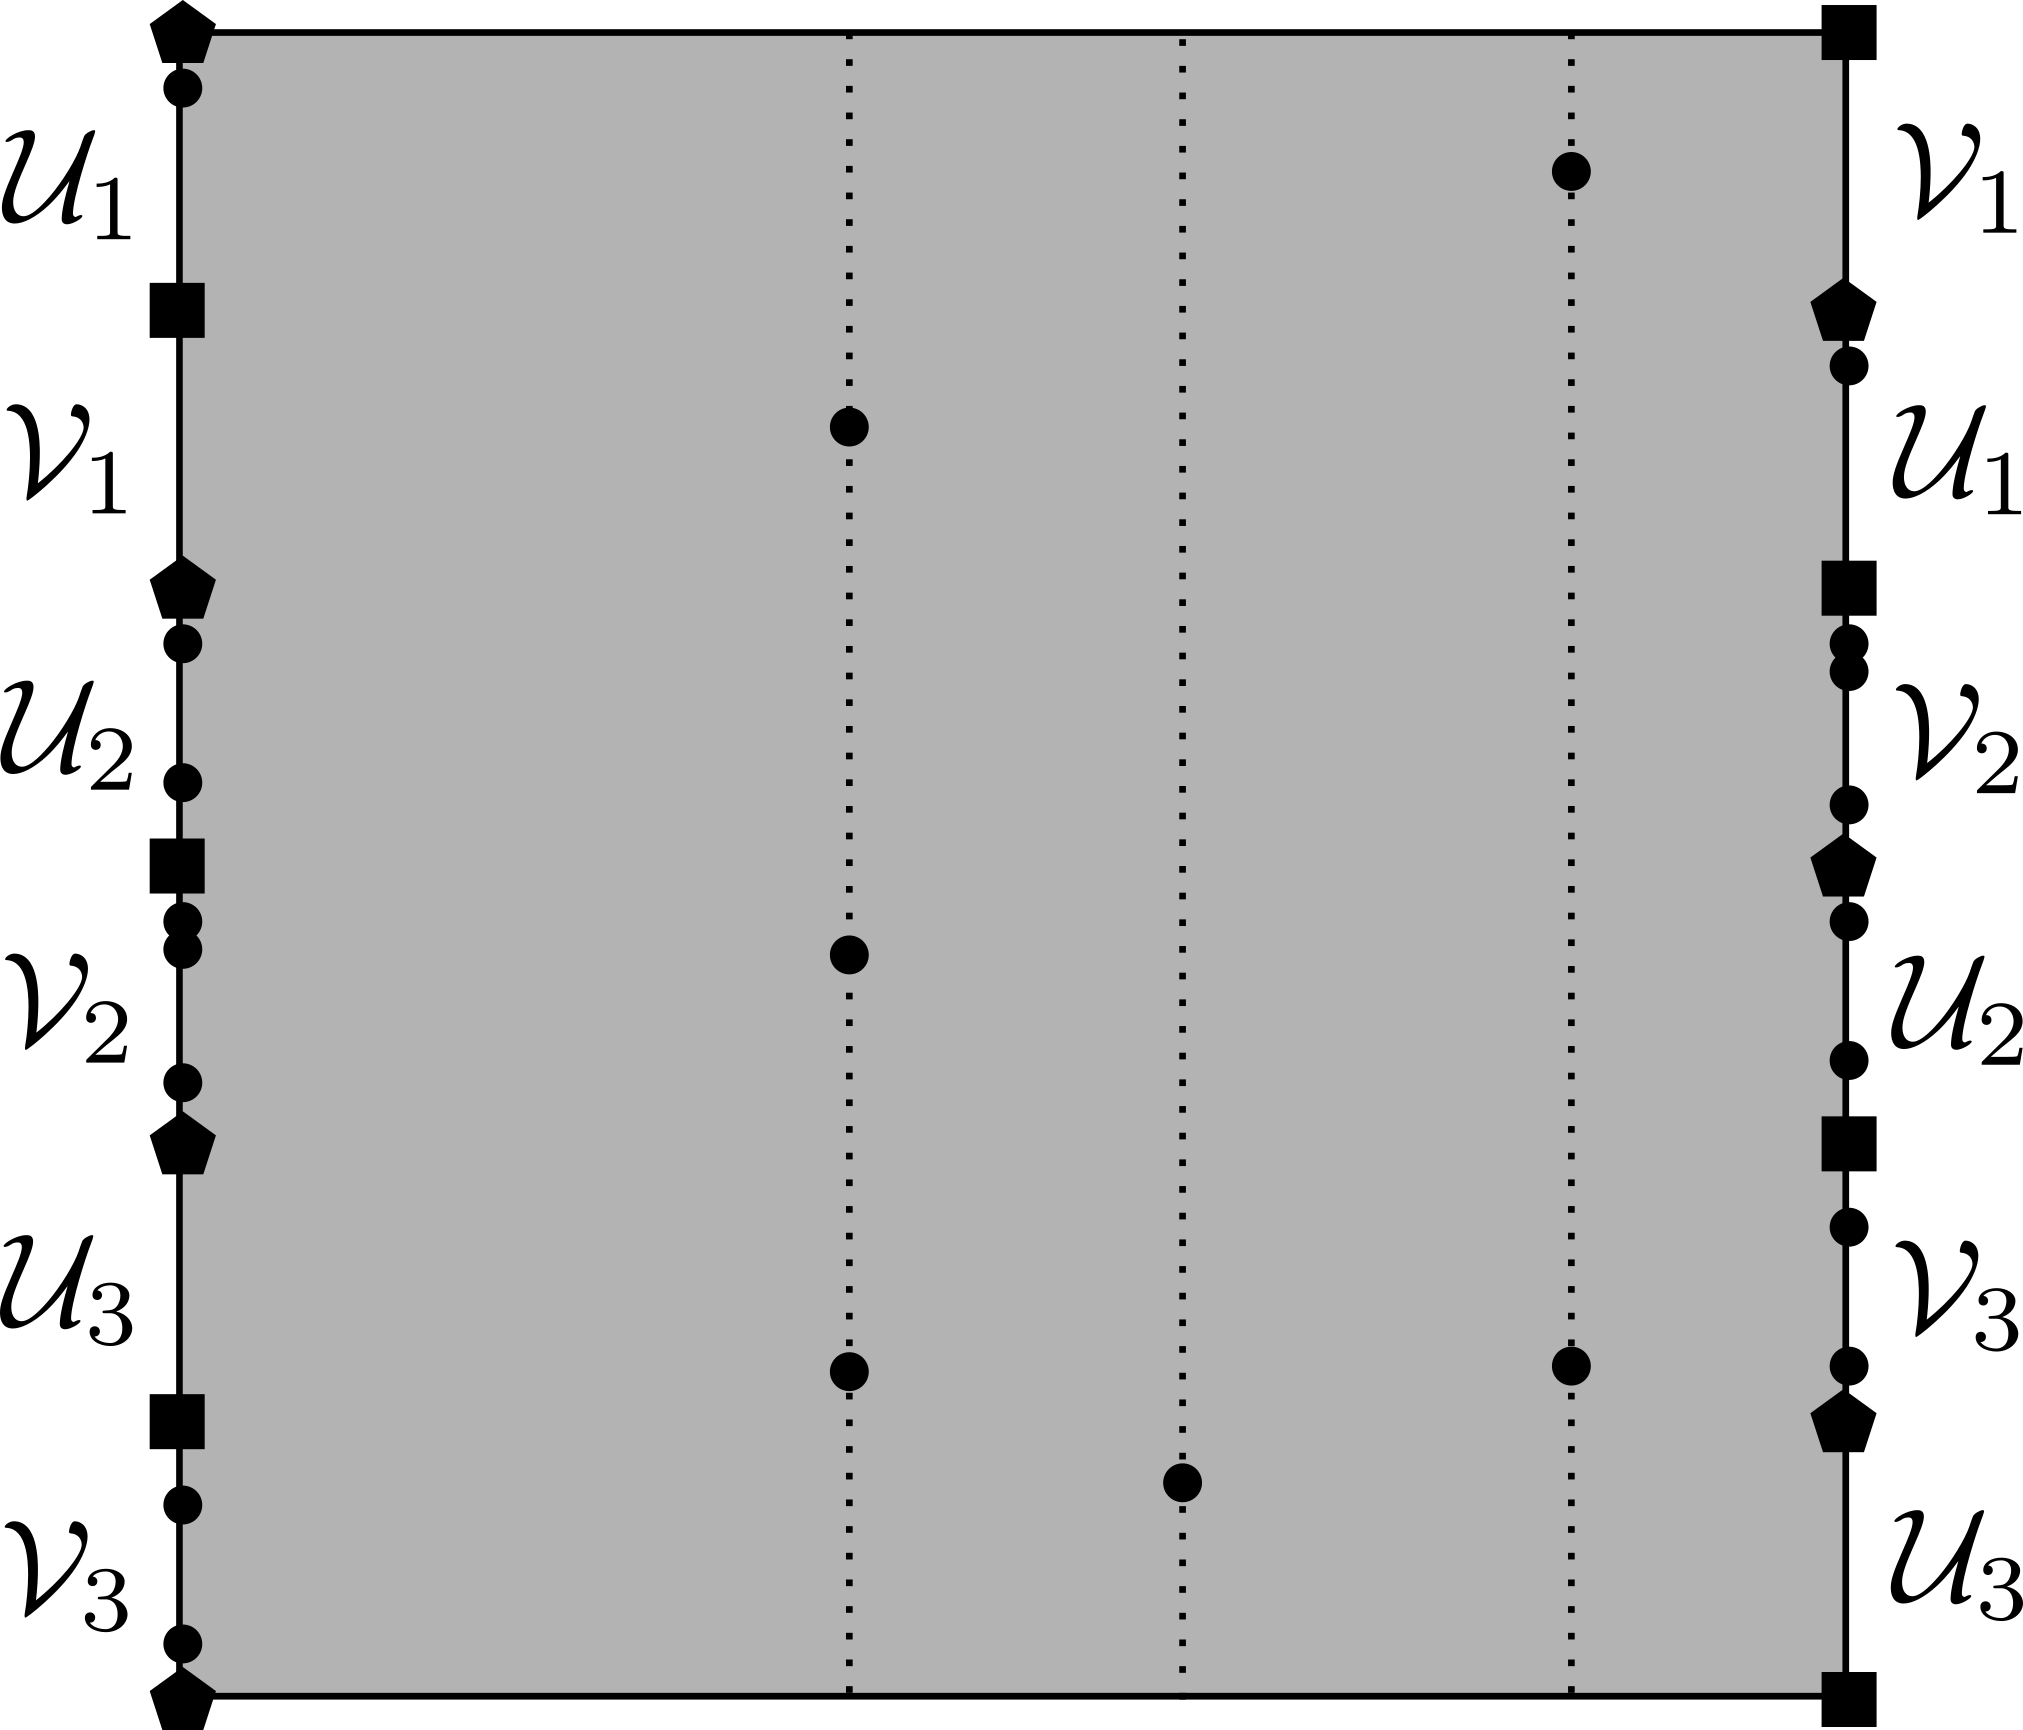
\includegraphics[scale=0.7]{figures/defetup.pdf}
 \caption{A configuration in the subspace $e^{\tup}\subset C_{14}(\S)$, for the tuple $\tup=(3,(3,1,2),(1,2,0),(0,3,2))$. Points
 lying on the $\U_i$'s and the $\V_i$'s are depicted twice.}
\label{fig:defetup}
\end{figure}


The space $e^{\tup}$ is homeomorphic to \emph{the interior} of the following multisimplex:

% We want to show that the collection of the $e_h$ for varying $h$, together with
% the 0-cell $*$, give a cell decomposition of $C_k(\S)^{\infty}$. Denote by $\Delta^h$ the following product of simplices
\[
 \Delta^{\tup}\colon =
 \Delta^l\times\prod_{i=1}^l\Delta^{x_i}\times\prod_{i=1}^g\pa{\Delta^{u_i}\times\Delta^{v_i}},
%  =\prod_{m\in\symb_l}\Delta^m.
\]
where the simplex $\Delta^r$ is the subspace of $[0,1]^r$ of sequences $0\leq \tau_1\leq\dots\leq\tau_r\leq 1$
(the numbers $\tau_1,\dots,\tau_r$ are the \emph{local coordinates} of the simplex). The homeomorphism is given
as follows:
\begin{itemize}
 \item the local coordinates of the $\Delta^l$-factor correspond to the positions $s_1,\dots,s_l$ of the vertical
 lines in $(0,1)^2$ containing points of the configuration;
 \item the local coordinates of the $\Delta^{x_i}$-factor correspond to the positions of the $x_i$ points
 lying on the vertical line $\set{s_i}\times(0,1)$;
 \item the local coordinates of the $\Delta^{u_i}$-factor correspond to the positions of the $u_i$ points
 lying on $\U_i$, which is canonically identified with $(0,1)$; similarly for the $\Delta^{v_i}$-factor,
 with $v_i$ and $\V_i$ replacing $u_i$ and $\U_i$.
\end{itemize}
Note that the dimension of $\Delta^{\tup}$ agrees with the dimension of $\tup$ from Definition \ref{defn:ehopen}.
The embedding $\mathring{\Delta}^{\tup}\cong e^{\tup}\hookrightarrow \cms^{\infty}$ extends to a continuous map
$\Phi^{\tup}\colon\Delta^{\tup}\to\cms^{\infty}$, so that the image of $\partial\Delta^{\tup}$ is contained in the union of
all subspaces $e^{\tup'}$ for tuples $\tup'$ of \emph{lower} dimension than $\tup$, together with the $0$-cell $\infty$.

The construction of the map $\Phi^{\tup}$ is as follows:
\begin{enumerate}
\item we identify the one-point compactification
$(\mrS)^{\infty}$ of $\mrS=\T(\S)$ as the quotient of $Q(\S)$ collapsing the boundary to a point $\infty$;
\item we consider the $m$-fold symmetric product $\SP^m\pa{(\mrS)^{\infty}}$ (see Definition \ref{defn:SP}): it contains 
as an \emph{open} subspace $\cms$, so we can identify $\cms^{\infty}$ as the quotient of $\SP^m\pa{(\mrS)^{\infty}}$ collapsing
the subspace $\SP^m\pa{(\mrS)^{\infty}}\setminus\cms$ to $\infty$;
\item the homeomorphism $\mathring{\Delta}^{\tup}\to e^{\tup}\subset\cms$ extends
now to a map $\Delta^{\tup}\to\SP^m\pa{[0,1]^2}$, that we can then further project to $\SP^m(Q(\S))$, then to
$ \SP^m\pa{(\mrS)^{\infty}}$ and then to $\cms^{\infty}$: the composition
is the map $\Phi^{\tup}$.
\end{enumerate}
In the last step we used the open inclusion $\cms\subset\SP^m\pa{\mrS}\subset\SP^m\pa{(\mrS)^{\infty}}$, which
induces a map $ \SP^m\pa{(\mrS)^{\infty}}\to\cms^{\infty}$ by quotienting to $\infty$ the closed subspace
$ \SP^m\pa{(\mrS)^{\infty}}\setminus \cms^{\infty}$.

We conclude that the collection of the $e^{\tup}$'s, together with the $0$-cell $\infty$,
gives a cell decomposition of $\cms^{\infty}$, with characteristic maps of cells $\Phi^{\tup}$.

We compute the \emph{reduced} cellular chain complex of $\cms^{\infty}$
with coefficients in $\Z_2$. It is a chain complex in $\Z_2$-vector spaces with basis given
by tuples $\tup$, which correspond to the cells $e^{\tup}$.
\begin{lem}
\label{lem:doperatoropenmodtwo}
Let $\tup=(l,\ux,\uu, \uv)$ and
$\tup'=(l-1,\ux',\uu',\uv')$
be tuples in consecutive dimensions $m+l$ and $m+l-1$. Denote by $[\tup\colon\tup']\in\Z_2$ the coefficient
of $\tup'$ in $\partial \tup$ in the reduced chain complex $\tilde\Ch_*(\cms^{\infty})$.
Then $[\tup:\tup']=0$ unless one, and exactly one, of the following situations occurs:
\begin{itemize}
 \item $l\geq 2$ and $\tup'$ is obtained from $\tup$ by decreasing $l$ by 1, setting $x'_i=x_i+x_{i+1}$
 for one value $1\leq i\leq l-1$, and shifting the values
 $x'_j=x_{j+1}$ for $i+1\leq j\leq l-1$. In this case we say that $\tup'$ is an \emph{inner boundary} of $\tup$, and
 we have
 \[
  [\partial \tup\colon\tup']=\binom{x_i+x_{i+1}}{x_i}\in\Z_2.
 \]
%  This binomial coefficient may be anyway equal to $0\in\Z_2$.
 \item $l\geq 1$ and $\tup'$ is obtained from $\tup$ by decreasing $l$ by 1, choosing a splitting of $x_1$
 in integers $\tildeu_i,\tildev_i\geq 0$
 \[
  x_1=\sum_{i=1}^g \pa{\tildeu_i+\tildev_i},
 \]
 setting $u'_i=u_i+\tildeu_i$ and $v'_i=v_i+\tildev_i$ for all $1\leq i\leq g$ and shifting the values
 $x'_j=x_{j+1}$ for $1\leq j\leq l-1$. In this case we say that $\tup'$ is a \emph{left, outer boundary} of $\tup$, and we have
 \[
  [\partial \tup\colon\tup']=\prod_{i=1}^g\binom{u_i+\tildeu_i}{u_i}\binom{v_i+\tildev_i}{v_i}\in\Z_2.
 \]
%  This product of binomial coefficients may be anyway equal to $0\in\Z_2$.
 \item $l\geq 1$ and $\tup'$ is obtained from $\tup$ by decreasing $l$ by 1, choosing a splitting of $x_l$
 in integers $\tildeu_i,\tildev_i\geq 0$
 \[
  x_l=\sum_{i=1}^g \pa{\tildeu_i+\tildev_i},
 \]
 setting $u'_i=u_i+\tildeu_i$ and $v'_i=v_i+\tildev_i$ for all $1\leq i\leq g$ and keeping $x'_i=x_i$ for all $1\leq i\leq l-1$.
 In this case we say that $\tup'$ is a \emph{right, outer boundary} of $\tup$, and we have
 \[
  [\partial \tup\colon\tup']=\prod_{i=1}^g\binom{u_i+\tildeu_i}{u_i}\binom{v_i+\tildev_i}{v_i}\in\Z_2.
 \]
%  This product of binomial coefficients may be anyway equal to $0\in\Z_2$.
\end{itemize}

\end{lem}
It may indeed happen that $\tup'$ is both a left and a right outer boundary of $\tup$,
namely when all numbers $(x_i)_{1\leq i\leq l}$ are equal; then the two contributions cancel each other,
so that $[\tup\colon\tup']=0$ as stated.
\begin{proof}
 For $1\leq i\leq l$ denote by $\partial^{\hor}_i\Delta^{\tup}$ the face
 \[
 \partial_i\Delta^l\times\prod_{i=1}^l\Delta^{x_i}\times\prod_{i=1}^g\pa{\Delta^{u_i}\times\Delta^{v_i}}\subset\Delta^{\tup}.
 \]
 This is also referred as the $i$-th \emph{horizontal face}. All other faces of codimension 1 of
 the multisimplex $\Delta^{\tup}$ are called \emph{vertical}.
 
 We note that $\Phi^{\tup}$ restricts to a cellular map $\partial_i^{\hor}\Delta^{\tup}\to\cms^{\infty}$ on every
 horizontal face, where $\partial_i^{\hor}\Delta^{\tup}$
 is given the cell structure coming from the multisimplicial structure: every subface of $\partial_i^{\hor}\Delta^{\tup}$ of dimension
 $k\leq m+l-1$ is mapped to the $k$-skeleton of $\cms^{\infty}$. Therefore the map $\Phi^{\tup}\colon\partial_i^{\hor}\Delta^{\tup}\to\cms^{\infty}$
 has a well-defined local index over the cell $e^{\tup'}$, that
 we call $[\partial^{\hor}_i\tup\colon\tup']\in\Z_2$.

 The same holds for vertical faces, where the restriction of $\Phi^{\tup}$ is the constant map to $\infty$: in this case the local index
 over $e^{\tup'}$ is zero. The index $[\tup\colon\tup']$ of the map $\Phi^{\tup}\colon\partial\Delta^{\tup}\to\cms^{\infty}$ on
 $e^{\tup'}$ splits as a sum of local indices:
 \[
  [\tup\colon\tup']=\sum_{i=0}^l[\partial_i^{\hor}\tup\colon\tup']\in\Z_2.
 \]
 For $0\leq i\leq l$ the restriction $\Phi^{\tup}\colon\partial^{\hor}_i\Delta^{\tup}\to\cms^{\infty}$
 hits homeomorphically the open cell $e^{\tup'}$
 exactly as many times as specified in the statement
 of the lemma for the cases $1\leq i\leq l-1$,
 $i=0$ and $i=l$ respectively.
 
 The only possibility in which the same cell $e^{\tup'}$ is hit by different faces $\partial_i^{\hor}\Delta^{\tup}$
 and $\partial_j^{\hor}\Delta^{\tup}$ is the one described in the remark preceding this proof: in this case
 there are two equal contributions $[\partial_i^{\hor}\tup\colon\tup']$ and $[\partial_j^{\hor}\tup\colon\tup']$
 that cancel each other.
%  We are working in $\Z_2$ so we do not have to be careful about orientations of cells
%  and therefore about signs.
\end{proof}

We can filter the reduced chain complex $\tilde\Ch_*(\cms^{\infty})$ by giving filtration norm $\sum_{i=1}^lx_i$ to
the tuple $\tup=(l,\ux,\uu,\uv)$, with $\ux=(x_1,\dots,x_l)$. For example
the tuple in Figure \ref{fig:defetup} has norm 6.

By Lemma \ref{lem:doperatoropenmodtwo}
the norm is weakly decreasing along differentials. Denote by $F_p\subset\tCh_*(\cms^{\infty})$ the subcomplex generated by
tuples of norm $\leq p$, and let $F_p/F_{p-1}$ be the $p$-th filtration stratum.
Then $F_p/F_{p-1}$ is isomorphic, as a chain complex, to a direct sum of copies of $\tCh_*(C_p(\Sigma_{0,1})^{\infty})$:
there is one copy for each partition
\[
(m-p)=\sum_{i=1}^g (u_i+v_i)
\]
with $u_i,v_i\geq 0$. The isomorphism
does not preserve the degrees but shifts them by $p$.

Indeed in $F_p/F_{p-1}$ all outer
differentials vanish (see Lemma \ref{lem:doperatoropenmodtwo}): in particular the numbers $u_i,v_i$
do not change along the differentials of $F_p/F_{p-1}$. Therefore $F_p/F_{p-1}$ splits as a direct sum
of chain complexes indexed by all partitions $(m-p)=\sum_{i=1}^g (u_i+v_i)$ as above.
It is then immediate to identify the inner faces
with the ones one would have in the case $g=0$, i.e. for the surface $\Sigma_{0,1}$, after shifting
degrees by $p$.

We note that $\tCh_*(C_p(\Sigma_{0,1})^{\infty})$ is exactly the chain complex described by Fuchs in
\cite{Fuchs:CohomBraidModtwo}: we recall Fuchs' computation of the cohomology of configuration
spaces of the disc, and abbreviate $\D$ for $\mathring{Sigma}_{0,1}$ as in Section \ref{sec:Preliminaries}.
\begin{defn}
\label{defn:symchain}
Consider a partition of $p$ into powers of 2
\[
 p=\sum_{j\geq 0}\alpha_j2^j,
\]
and let $\ualpha=(\alpha_j)_{j\geq 0}$ be the sequence of multiplicities. We understand that only finitely
many $\alpha_j$'s are strictly positive.

The associated \emph{symmetric chain} in $\tCh_*(C_p(\D)^{\infty})$, denoted by $\kappa(\ualpha)$,
is the sum of all tuples $\tup=\pa{l,(x_i)_{i\leq l}}$ such that
\begin{itemize}
 \item $l=\sum_{j\geq 1}\alpha_j$;
 \item every $x_i$ is a power of 2;
 \item for all $j\geq 0$ there are exactly $\alpha_j$ indices $i$ such that $x_i=2^j$.
\end{itemize}
% Here and in the following it is understood that $\alpha_j=0$ for all but finitely many indices $j$.
A symmetric chain $\kappa(\ualpha)$ is a cycle in the chain complex $\tCh_*(C_p(\D)^{\infty})$ (see \cite{Fuchs:CohomBraidModtwo}).
We denote by $[\kappa(\ualpha)]\in\tH_{p+l}(C_p(\D)^{\infty})$ the associated homology class.
\end{defn}
In \cite{Fuchs:CohomBraidModtwo} Fuchs shows that a graded basis for $\tH_*(C_p(\D)^{\infty})$
is given by the collection of all classes $[\kappa(\ualpha)]$ associated to sequences $\ualpha=(\alpha_j)_{j\geq 0}$
which satisfy the equality $p=\sum_{j\geq 0}\alpha_j2^j$.

By Poincaré-Lefschetz duality this corresponds to a basis for $H^*(C_p(\D))$.
The \emph{dual} basis of $H_*(C_p(\D))$
happens to be the basis of monomials
\[
Q^{\ualpha}\epsilon\colon =\prod_{j\geq 0}(Q^i\epsilon)^{\alpha_j}\in H_*(C_p(\D)).
\]
This basis consists of all monomials
of weight $p$, using
the isomorphism \eqref{eq:Cohen} in its full meaning (i.e. as an isomorphism of rings,
where $Q$ denotes the first Dyer-Lashof operation).

% This notation is compatible, after interpreting equation \eqref{eq:genuszero} as an isomorphism
% of rings, with the results of \cite[Chap.3]{CLM}: the monomials constructed there, using
% the Pontryagin product and the operation $Q$, are really the dual basis of the basis of
% symmetric chains for cohomology.

We will not need this finer result in this article, so in the following the expression
$Q^{\ualpha}$ will only denote
the (unique) homology class in $H_{p-l}(C_p(\D)$ such that the following holds:
for all $\ualpha'=(\alpha'_j)_{j\geq 0}$ with $\sum_{j\geq 0}\alpha'_j=p$, the
algebraic intersection between $Q^{\ualpha}\epsilon\in H_{p-l}(C_p(\D))$
and $[\kappa(\ualpha')]\in\tH_{p+l}(C_p(\D)^{\infty})$
is $1\in\Z_2$ if and only $\ualpha=\ualpha'$.
% i.e. we \emph{define} monomials as the dual basis of the basis of symmetric chains, and keep considering
% \eqref{eq:Cohen} only as an isomorphism of bigraded vector spaces.

We now go back to the filtered chain complex $\tCh_*(\cms^{\infty})$.
The $E^1$-page of the associated Leray spectral sequence contains on the $p$-th column
the homology of $F_p/F_{p-1}$; as we have seen the homology of this filtration stratum is
the direct sum of several copies of the homology of $\tCh_*(C_p(\D))$, one copy for each
partition $(m-p)=\sum_{i=1}^g (u_i+v_i)$ with $u_i,v_i\geq 0$.

\begin{defn}
\label{defn:gensymchain}
Consider a partition
\[
 m=p+(m-p)=\pa{\sum_{j=0}^{\infty}\alpha_j2^j}+\pa{\sum_{i=1}^g(u_i+v_i)}
\]
and let $\uu=(u_1,\dots,u_g)$, $\uv=(v_1,\dots, v_g)$, $\ualpha=(\alpha_j)_{j\geq 0}$; denote also $l=\sum_{j=1}^{\infty}\alpha_j$.

We define a chain $\kappa(p,\ualpha,\uu,\uv)$ in
$\tCh_{m+l}(\cms)$: it
is the sum of all tuples $\tup$ of the form $\pa{l,\ux,\uu,\uv}$, for varying $\ux$,
which satisfy the three properties listed in Definition \ref{defn:symchain}.

We call such a chain a
\emph{generalised symmetric chain}; we will see in the following that it is a cycle, and we will
denote by $[\kappa(p,\ualpha,\uu,\uv)]$ the associated homology class in $\tH_{m+l}(\cms^{\infty})$.

If any of $\ualpha$, $\uu$ and $\uv$ vanishes, we omit it from the notation.
\end{defn}

A generalised symmetric chain $\kappa(p,\ualpha,\uu,\uv)$
is not only
a cycle when projected to its filtration quotient $F_p/F_{p-1}$, as the $E^1$-page
of the spectral sequence tells us, but also
in the chain complex $\tCh_*(\cms^{\infty})$ itself.

To prove this fact, first note that an inner boundary of a tuple
$\tup$ preserves the norm; hence the fact that $\kappa(p,\ualpha,\uu,\uv)$ is a cycle
in $F_p/F_{p-1}$ guarantees the fact that all inner boundaries of $\kappa(p,\ualpha,\uu,\uv)$
cancel each other in $\tCh_*(\cms^{\infty})$, that is,
\[
\partial\kappa(p,\ualpha,\uu,\uv)\in \tCh_*(\cms^{\infty})
\]
is equal to the sum of all outer boundaries of the tuples involved.

Note now that outer boundaries of a generalised symmetric chain also cancel out:
the left outer boundary
of a tuple $\tup=(l,\ux,\uu,\uv)$ in the generalised symmetric chain cancels against the right outer boundary
of the tuple $\tup'=(l,\ux',\uu,\uv)$, with $x'_l=x_1$ and $x'_i=x_{i+1}$ for $1\leq i\leq l-1$. If all
$x_i$ happen to be equal, then $\tup=\tup'$ and
we are in the situation described before the proof of Lemma \ref{lem:doperatoropenmodtwo}.

The spectral sequence considered above collapses on its first page and
% $H_*(\cms^{\infty})$
% has a $\Z_2$-basis given by generalised symmetric chains.
we have the following lemma:
\begin{lem}
\label{lem:gensymchain}
The homology $H_*(\cms^{\infty})$ has a graded basis given by the classes $[\kappa(p,\ualpha,\uu,\uv)]$
associated to generalised symmetric chains of weight $m$.
% this basis is bijection with
% the choices of the following set of data:
% \begin{itemize}
%  \item a number $0\leq p\leq m$;
%  \item a splitting $m-p=\sum_{i=1}^g (u_i+v_i)$ with $u_i,v_i\geq 0$;
%  \item a splitting $p=\sum_{j=0}^{\infty}\alpha_j2^j$ with $\alpha_j\geq 0$.
% \end{itemize}
% The homology class $[p,(u_i,v_i),(\alpha_j)]\in H_*(\cms^{\infty})$ has homological degree
% $m+\sum_{j=1}^{\infty}\alpha_j$.
\end{lem}
% To interpret this class
% as a monomial in the tensor product of Theorem \ref{thm:Hbms*as*ggrep} we need the following definition.

% We are almost ready to prove an isomorphism of bigraded $\Z_2$-vector spaces as in Theorem \ref{thm:Hbms*as*ggrep}.

\begin{defn}
 \label{defn:dualHbasis}
We can see the $\U_i$'s and $\V_i$'s as properly embedded $1$-manifolds in $\mrS$;
by Poincaré-Lefschetz duality they represent classes in $\tH_1\pa{(\mrS)^{\infty}}\simeq H^1(\S)$,
and in particular they form a basis
of the latter cohomology group. We call $\u_i,\v_i\in H_1\pa{\mrS}$ the dual basis.

% We fix simple closed curves $\u_i,\v_i$ on $\S$, for $1\leq i\leq g$, whose fundamental classes
% $[\u_i],[\v_i]$ form the dual basis of $H_1(\S)$. We assume that, apart from the following necessary exceptions,
% all curves $\U_i,\V_i,\u_i,\v_i$ for $1\leq i\leq g$ are disjoint:
% \begin{itemize}
%  \item $\u_i$ and $\v_i$ intersect once, transversely;
%  \item $\u_i$ and $\U_i$ intersect once, transversely;
%  \item $\v_i$ and $\V_i$ intersect once, transversely;
%  \end{itemize}
% SEE PICTURE.
\end{defn}
We establish a bijection between monomials in the tensor product of Theorem \ref{thm:Hbms*as*ggrep}
and the basis of $H^*(\cms)\simeq H_*(\cms^{\infty})$ in Lemma \ref{lem:gensymchain}:
the class 
\[
[\kappa(p,\ualpha,\uu,\uv)]\in H_{m+\sum\alpha_j}(\cms^{\infty})\simeq H^{m-\sum\alpha_j}(\cms)
\]
is associated with the monomial
\[
Q^{\ualpha}\epsilon\cdot\u^{\uu}\cdot\v^{\uv}\colon =\prod_{j=1}^{\infty}(Q^j\epsilon)^{\alpha_j}\otimes \prod_{i=1}^g(\u_i^{u_i}\v_i^{v_i}),
\]
where $\ualpha=(\alpha_j)_{j\geq 0}$, $\uu=(u_1,\dots,u_g)$ and $\uv=(v_1,\dots,v_g)$.

This shows an isomorphism of bigraded $\Z_2$-vector spaces
\begin{equation}\label{eq:isovectorspaces}
  \bigoplus_{m\geq 0} H^*(\cms)\simeq \Z_2\left[Q^j\epsilon\,|\, j\geq 0\right]\otimes\Sym_{\bullet}(\H),
\end{equation}
from which we conclude that
there exists an isomorphism as in Theorem \ref{thm:Hbms*as*ggrep}
at least \emph{as bigraded $\Z_2$-vector spaces}: the two bigraded
vector spaces have the same dimension in all bigradings.